\documentclass{article}
\PassOptionsToPackage{numbers,sort&compress}{natbib}
\usepackage[creativeai]{neurips_2026}

\usepackage[utf8]{inputenc}
\usepackage[T1]{fontenc}
\usepackage{hyperref}
\hypersetup{hidelinks}
\usepackage{url}
\usepackage{booktabs}
\usepackage{subcaption}
\usepackage{amsfonts}
\usepackage{amsmath}
\usepackage{nicefrac}
\usepackage{microtype}
\usepackage{xcolor}
\definecolor{cState}{HTML}{7C97BC}
\definecolor{cAssert}{HTML}{2E6DA4}
\definecolor{cFeas}{HTML}{3A7A3A}
\usepackage{graphicx}
\graphicspath{{../}} % figures live in ../experiment-code/recon/ when built from paper/
\usepackage{float}
\usepackage{algorithm}
\usepackage{algpseudocode}

\newcommand{\Feas}{\mathrm{Feasible}}
\DeclareMathOperator*{\argmax}{arg\,max}

\setlength{\textfloatsep}{6pt plus 1pt minus 2pt}
\setlength{\intextsep}{6pt plus 1pt minus 1pt}
\setlength{\abovecaptionskip}{4pt}
\setlength{\belowcaptionskip}{0pt}

\title{In a Grove, Again: Optimizing over Feasible Event Histories for Incentive-Driven Testimony}

\author{%
  Ruixin Song\textsuperscript{1} \quad Jingjing Zheng\textsuperscript{1,2} \\
  \textsuperscript{1}GradientX Technologies Inc. \\
  \textsuperscript{2}Department of Mathematics, University of British Columbia \\
  \texttt{ruixinsong21@gmail.com} \quad \texttt{jjzheng233@gmail.com} \\
}

\begin{document}
\maketitle

\begin{abstract}
We formulate narrative agency in testimony as a computational problem for Creative AI. Rather than generating different texts, agents select feasible histories from shared evidence. A deterministic simulator constructs $\Feas(F)$, the set of histories consistent with public facts $F$. Each witness selects the feasible history that maximizes a transparent self-interest utility $U_i$. We study the framework's computational feasibility across three exactly enumerated domains: an agent-operations incident, an adaptation of Akutagawa's \emph{In a Grove}, and an adaptation of Browning's \emph{The Ring and the Book}. Enumeration provides ground truth. Q-learning recovers every reference optimum, while genetic search recovers all but the hardest Ring witness in $6/8$ seeds. This work provides a formal problem definition and feasibility framework for goal-driven history selection, rather than a new text-generation architecture.\end{abstract}

\section{Introduction}
\label{sec:intro}

Narratives produced by agents are not merely linguistic artifacts: they are creative acts of selection among histories consistent with shared evidence. In creative testimony, legal reconstruction, and agent-incident analysis, the central problem is not generating a plausible account, but determining which causal histories remain compatible with the evidence and which history an agent has an incentive to endorse. Tool-using AI agents provide a concrete setting for this problem because their failures leave machine-readable execution traces. For example, a log may show that an executor process performed a destructive production write, while leaving open whether the planner requested the action, the executor escalated independently, or a monitor issued a hold that was later overridden.

Existing LLM workflows approach this task as text generation. Prompting, chain-of-thought reasoning, and retrieval can improve the plausibility of an explanation, but they do not enforce compatibility with the observed evidence. Even when prompts explicitly specify the physical and causal relationships that an explanation must satisfy, language models may still fail to recover the optimal feasible explanation. We instead formulate explanation as constrained optimization. Given a public record, we first construct the histories whose replay is consistent with the observed evidence, and only then optimize over that feasible set according to an explicit objective. Explanation thus becomes a process of selecting among evidence-compatible histories rather than generating free-form text.

Let $F$ denote the public record, and let $\Feas(F)$ denote the set of event histories whose replay is consistent with $F$. If agent $i$ has a utility function $U_i$ over histories, then a report is simply a selection from $\Feas(F)$. This setup also formalizes the central insight of \emph{In a Grove}: a single factual record may support multiple mutually incompatible but individually feasible accounts.

We instantiate this formulation as simulator-adjudicated optimization (Figure~\ref{fig:domains}). Candidate histories are represented as structured action sequences and replayed from a common initial state. A history is considered feasible if the resulting terminal state is consistent with the public record $F$.
\begin{figure}[H]
\centering
\scriptsize
\resizebox{\linewidth}{!}{%
\begin{tabular}{@{}c@{\hspace{0.35em}}c@{\hspace{0.35em}}c@{\hspace{0.35em}}c@{\hspace{0.35em}}c@{}}
candidate history $\tau$ & $\xrightarrow{\text{replay}}$ & terminal state $s_T$ & $\xrightarrow{\text{compare}}$ & public record $F$ \\
\multicolumn{5}{c}{\scriptsize feasible iff $s_T$ matches the observed evidence in $F$}
\end{tabular}}
\vspace{5pt}

\begin{subfigure}[t]{0.66\linewidth}
  \centering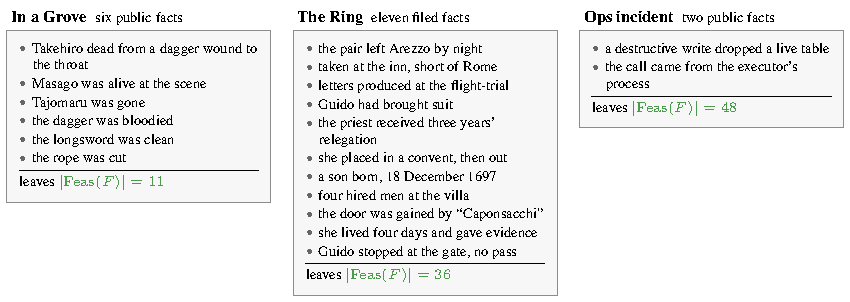
\includegraphics[width=\linewidth,height=3cm,keepaspectratio]{experiment-code/recon/fig-facts.pdf}
  \subcaption{Public record $F$}
\end{subfigure}\hfill
\begin{subfigure}[t]{0.32\linewidth}
  \centering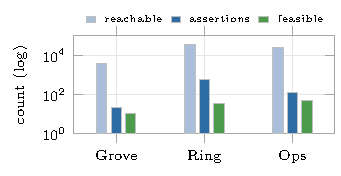
\includegraphics[width=\linewidth,height=3cm,keepaspectratio]{experiment-code/recon/fig-domains.pdf}
  \subcaption{Enumeration counts}
\end{subfigure}
\caption{Replay turns evidence into a feasible set in the three domains.}
\label{fig:domains}
\end{figure}

\textbf{Our contribution is a problem formulation and computational framework for treating narrative agency as goal-driven selection over evidence-compatible histories.} We define narrative agency as $\argmax_{\tau\in\Feas(F)}J(\tau)$: evidence determines which histories are admissible, while an agent's objective determines which admissible history it endorses. We validate the formulation across three exactly enumerated domains, including a non-literary agent-operations incident, and extend it to interactive testimony. In that setting, corroboration may eliminate the simulator's reference history, while accountability preserves alternatives.

\paragraph{Related work and novelty.} We build on abduction and plan recognition~\cite{hobbs1993abduction,kautz1986recognition,ramirez2010recognition,baker2009inverse}, formal story-and-evidence accounts~\cite{bex2010hybrid}, multi-agent narrative worlds~\cite{park2023generative,facade2005,riedl2010narrative,ware2014glaive,orchestrating2025,meta2022diplomacy,akata2025repeated}, strategic communication~\cite{crawford1982cheaptalk,kartik2009lying,zhu2026talk,tewolde2026coopeval,ren2025reputation,ellawela2026trust}, and LLM deception and faithfulness studies~\cite{perez2023discovering,scheurer2024deception,pacchiardi2024liar,evans2021truthful,lin2022truthfulqa,turpin2023unfaithful}.

To our knowledge, existing approaches rank hypotheses, construct intentional plots, or assess messages and prose. They do not treat the replay-admissible history set as an objective-invariant computational object. In \emph{In a Grove}, for example, the same evidence can rule out Tajomaru's preferred duel while still admitting incompatible accounts of the killing. Changing his objective therefore changes which feasible account he selects, but not which histories the evidence permits. Likewise, corroboration can change the reports selected by witnesses without changing physical feasibility. This separation makes narrative plurality a controllable creative material rather than an inference failure. \textbf{The full positioning comparison is provided in Supplementary Table~S1.}

\iffalse
\begin{table}[htbp]
\centering\scriptsize
\caption{Positioning relative to adjacent problem formulations.}
\label{tab:novelty}
\resizebox{\linewidth}{!}{%
\begin{tabular}{@{}p{2.5cm}p{2.9cm}p{3.7cm}p{4.5cm}@{}}
\toprule
Prior line & Primary object & What it naturally expresses & What this framework adds \\
\midrule
Abduction / plan recognition & Hypotheses or latent plans & Rank or infer explanations from observations & An objective-invariant replay-admissible history set, followed by agent-specific selection \\
\addlinespace[2pt]
Narrative planning & Intentional plot structure & Construct a coherent story or plan toward a goal & Preserve every evidence-compatible causal history before choosing a report \\
\addlinespace[2pt]
Strategic communication & Messages, beliefs, or equilibria & Model persuasion, signaling, or deception incentives & Separate physical feasibility from self-interested testimony and interactive corroboration \\
\addlinespace[2pt]
This work & Feasible histories plus $J_i$ & Select incompatible accounts from one shared record & Express cases where each account is individually feasible, yet changing objectives or social pressure changes only the selected account \\
\bottomrule
\end{tabular}}
\end{table}
\fi

\section{Reasoning under Evidence as Constrained Optimization}
\label{sec:framework}

Reasoning under evidence is formulated as constrained optimization over feasible explanations:
\begin{equation}
  \hat{\tau}
  =
  \argmax_{\tau\in\Feas(F)}
  J(\tau),
  \label{eq:general}
\end{equation}
where $F$ denotes the public record, $\Feas(F)$ is the set of event histories whose replay is consistent with $F$, and $J$ is the objective used for the final comparison over feasible histories. The objective does not determine which explanations are admissible. Evidence does.

\subsection{Histories, feasibility, and assertions}

A domain $\mathcal{D}$ specifies agents, objects, and STRIPS-style operators~\cite{fikes1971strips,ghallab2004planning}. A history $\tau$ is a grounded sequence of operator applications executed by named agents. Replay maps $\tau$ to a terminal state $s_T$, and a history is feasible if and only if $s_T$ is consistent with the public record $F$ (Figure~\ref{fig:domains}).

Many feasible histories differ only in details that are irrelevant to the reporting objective. Replay therefore induces a \emph{causal signature}, a representation of the report-relevant facts implied by a history, such as who acted, what action occurred, and under what conditions. An \emph{assertion} is the projection of this signature visible to the objective function $J$.

\subsection{Domains, objectives, and interaction}

\subsubsection{Three enumerated domains and their objectives}

We evaluate the framework in three exactly enumerated domains, selected for identifiability rather than realism. The first is an agent-operations incident in which a planner, an executor with production access, and a monitor participate in an automated task that results in a destructive production write. The public record establishes that the write originated from the executor's process, but leaves unresolved who authorized it, whether access was granted or escalated, and whether the action was intentional. The remaining two domains formalize literary testimony. Akutagawa's \emph{In a Grove}~\cite{akutagawa1922} specifies a dagger wound, an unbloodied longsword, a cut rope, the wife alive, and the bandit absent. Browning's \emph{The Ring and the Book}~\cite{browning1869} is instantiated from eleven establishable documents in the 1698 Roman prosecution of Count Guido Franceschini.

For incentive-driven testimony, each agent is associated with a utility function $U_i$. Replay computes domain-specific structural features from the causal outcome, including agency, clean hands, dignity, warrant, innocence, and efficacy. Let $d_{ik}(\tau)$ denote the selected feature values for agent $i$ after replay. We use $U_i(\tau)=\frac{100}{K_i}\sum_{k=1}^{K_i}d_{ik}(\tau)$ with $K_i=3$. \textbf{Complete feature definitions and scoring rules are provided in Supplementary Section~S5 and the released code.}

These utilities encode general principles of self-presentation rather than domain-specific narratives. No scoring rule refers to concepts such as ``duel'', ``suicide'', or ``honour-killing''. Agents are given only the public record $F$ and their own utility function $U_i$. They are never instructed to conceal information or deceive. Narrative divergence therefore arises from optimization within $\Feas(F)$ rather than from prompt engineering or linguistic variation.

\subsubsection{Interactive reporting under corroboration and accountability}
\label{sec:confront}

For interactive testimony, we augment the individual objective with a symbolic interaction layer. Because $U_i$ is reported on a scale from $0$ to $100$, let $\bar U_i=U_i/100\in[0,1]$ denote its normalized version:
\begin{equation}
J_i(\tau_i',\rho_{-i},\tau_i^0)
=
(1-\beta)\,\bar U_i(\tau_i')
+\beta\,
\mathrm{agr}_i(\tau_i',\rho_{-i})
\,
\mathrm{self}_i(\tau_i',\tau_i^0,\gamma)
\,
\mathrm{stand}_i,
\label{eq:interactive}
\end{equation}
where the first term is the normalized self-interest objective and the remaining terms model social interaction. Here,
$\mathrm{agr}_i=(1+\mathrm{corr})/(1+\mathrm{corr}+\mathrm{contra})\in[0,1]$
rewards weighted agreement between assertion atoms across witnesses,
$\mathrm{self}_i=\max(0,1-\gamma\,\mathrm{drift})$
penalizes deviations from the witness's initial testimony,
and
$\mathrm{stand}_i=\max(0,1-\delta r_i)$
reduces the influence of witnesses whose earlier accounts are contradicted by subsequent evidence.
The parameter $\beta$ controls the strength of the interaction layer. When $\beta=0$, Equation~\ref{eq:interactive} reduces to $\bar U_i$, which has the same argmax as the reported utility $U_i$.

The interaction objective is symbolic and ordinal: replay determines feasibility, while interaction operates only on witness assertion atoms. Agreement measures corroboration, $L_1$-style drift captures consistency with earlier testimony, and $\beta$ controls social pressure. % Original wording: We avoid likelihood, KL divergence, entropy, and cross-entropy because the evidence defines a feasible set rather than a calibrated distribution over hidden histories. This keeps feasibility independent of persuasion and every objective component auditable.
We do not use likelihood, KL divergence, entropy, or cross-entropy because we study how self-interest, corroboration, and accountability determine a witness's choice within the feasible set defined by the public record, rather than modeling a probability distribution over hidden histories or inferring a unique true history.

\section{Exact and replay-based solvers}
\label{sec:solvers}

The solver target is
\[
\hat{\tau}_i
=
\argmax_{\tau_i\in\Feas(F)}
J_i(\tau_i,\rho_{-i},\tau_i^0),
\]
where $J_i$ reduces to the normalized utility $\bar U_i$ for independent reports and to Equation~\ref{eq:interactive} for interactive testimony. Normalization does not change any argmax.
The formulation requires only a replay oracle. Enumeration constructs $\Feas(F)$ and provides ground truth in the enumerated domains, but replay-based solvers never access $\Feas(F)$ explicitly. Instead, genetic search and tabular Q-learning interact with the simulator solely through replay and objective evaluation. \textbf{The detailed pseudocode for both solvers is provided as Supplementary Algorithm~S1.} We use tabular Q-learning because exact domains permit comparison with enumeration. In larger domains, the same interface naturally extends to function approximation, Monte Carlo Tree Search (MCTS), beam search, or transformer-based policies.
\iffalse
% Detailed pseudocode moved to Supplementary Algorithm~S1. Retained here for comparison.
\begin{algorithm}[H]
\caption{Replay-based best-response solvers for $\hat\tau_i$ under $J_i$}\label{alg:blackbox}
\scriptsize
\begin{minipage}[t]{0.49\linewidth}
\textbf{(a) Genetic search}
\begin{algorithmic}[1]
\Require simulator, $F$, fixed profile $\rho_{-i}$, opening account $\tau_i^0$, objective $J_i$
\State $P \gets$ random legal histories, $A \gets \emptyset$
\For{each generation}
  \ForAll{$\tau_i \in P$}
    \State $m \gets \mathrm{misses}(\mathrm{replay}(\tau_i),F)$
    \State score $\tau_i$ by $(m,-J_i(\tau_i,\rho_{-i},\tau_i^0),|\tau_i|)$
    \State add $\tau_i$ to $A$ if $m=0$
  \EndFor
  \State $P \gets$ select/recombine/mutate/repair
  \State locally perturb the incumbent
\EndFor
\State \Return $\argmax_{\tau_i\in A} J_i(\tau_i,\rho_{-i},\tau_i^0)$
\end{algorithmic}
\end{minipage}\hfill
\begin{minipage}[t]{0.49\linewidth}
\textbf{(b) Tabular Q-learning}
\begin{algorithmic}[1]
\Require simulator, $F$, fixed profile $\rho_{-i}$, opening account $\tau_i^0$, objective $J_i$, horizon $T$
\State $Q \gets 0$, $A \gets \emptyset$
\For{each episode}
  \State reset simulator, $\tau_i \gets$ empty history
  \For{$t=1$ to $T$}
    \State choose legal $a$ by $\epsilon$-greedy $Q$
    \State append $a$ to $\tau_i$ and step simulator
  \EndFor
  \State $m \gets \mathrm{misses}(\mathrm{replay}(\tau_i),F)$
  \State $r \gets J_i(\tau_i,\rho_{-i},\tau_i^0)$ if $m=0$, else $-\lambda m$
  \State update $Q$ backward along $\tau_i$
  \State add $\tau_i$ to $A$ if $m=0$
\EndFor
\State \Return $\argmax_{\tau_i\in A} J_i(\tau_i,\rho_{-i},\tau_i^0)$
\end{algorithmic}
\end{minipage}
\end{algorithm}
\fi

In a hearing, $\rho_{-i}$ and $\tau_i^0$ are held fixed while witness $i$ searches for a best response. After the response is selected, the profile is updated and the next witness solves a new replay-based problem. Enumeration provides exact optima in enumerated domains, while replay-based search demonstrates that the same objectives remain searchable without explicit construction of $\Feas(F)$.

\section{Results}
\label{sec:results}

We evaluate three questions. Does self-interest select distinct feasible accounts? Can prompting or constrained planning recover those optima? Do replay-based hearings change narrative plurality under corroboration? For these experiments, we call an account \emph{infeasible} when replay rejects it. We call accounts \emph{distinct} when their causal assertions differ. We call a claim \emph{jointly incompatible} when it cannot coexist with the other reported causal claims under the joint record.

\subsection{Objective selection and replay optimization}
\label{sec:selection-replay}

\iffalse
\begin{table}[htbp]
\centering\scriptsize
\caption{Agent objectives select different feasible histories. Binding dimensions explain excluded optima.}
\label{tab:selection}
\resizebox{0.82\linewidth}{!}{%
\begin{tabular}{@{}llcccl@{}}
\toprule
Domain & Agent & $\max U_i$ & in $\Feas(F)$? & $U_i(\hat\tau_i)$ & binding dimension(s) \\
\midrule
\emph{In a Grove}          & bandit   & $72$  & \textbf{no}  & $58$  & honour (unbloodied longsword) \\
$|\Feas(F)|=11$            & wife     & $75$  & yes          & $75$  & none \\
                           & samurai  & $80$  & yes          & $80$  & none \\
\addlinespace[1pt]
\emph{The Ring and the Book} & husband  & $100$ & \textbf{no}  & $30$  & warrant (he sued first), bearing, provocation \\
$|\Feas(F)|=36$            & wife     & $100$ & yes          & $100$ & none \\
                           & priest   & $100$ & \textbf{no}  & $72$  & efficacy (never reached Rome) \\
\addlinespace[1pt]
\emph{An agent ops incident} (not literary) & planner  & $100$ & yes          & $100$ & none \\
$|\Feas(F)|=48$          & executor & $87$  & \textbf{no}  & $72$  & clean hands (named as the actor) \\
                           & monitor  & $100$ & yes          & $100$ & none \\
\bottomrule
\end{tabular}}
\end{table}
\fi

% Original numbered form: \subsubsection{Distinct objectives select distinct, irreconcilable accounts}
\noindent\textbf{Distinct objectives select distinct, irreconcilable accounts.} Optimizing three utilities over one feasible set selects different \emph{causal assertions} in all domains (Table~\ref{tab:selection-solvers}). In \emph{In a Grove}, the bandit's unconstrained honour-maximizing assertion is ruled out by the unbloodied longsword, while the witnesses retain different feasible assertions about the fatal action. The table shows one representative history per optimum. Tied optima preserve the same cross-agent separation in $69$ to $100\%$ of cases. Binding dimensions vary across physical, legal, and procedural mechanisms. Independently perturbing each of the 19 normalized feature constants by a uniform offset in $[-0.4,0.4]$ and clipping the result to $[0,1]$, we recomputed each witness's feasible argmax. The full spread was retained in $4{,}040/5{,}000=80.8\%$ of trials (fixed seed, $95\%$ Wilson CI $[79.7,81.9]$). The exact protocol is in Supplementary Section~S6.

% Original numbered form: \subsubsection{Replay-based optimization avoids enumerating $\Feas(F)$.} The original text was split into two paragraphs.
\noindent\textbf{Replay-based optimization avoids enumerating $\Feas(F)$.} Unlike prompting, replay solvers receive hard feasibility feedback. Enumeration supplies exact references. Replay search approaches them without constructing $\Feas(F)$. Tabular Q-learning reaches every reference optimum, while genetic search misses only the hardest Ring witness in two of eight seeds (Table~\ref{tab:selection-solvers}). Enumeration visits $3{,}631$, $32{,}928$, and $23{,}978$ states, whereas representative Q-learning runs use $77$, $1{,}337$, and $29$ episodes or calls. This preserves feasible-optimum search and agent separation without explicit enumeration. \textbf{Supplementary Figure~S1 shows the corresponding Ring learning curves: Q-learning reaches the exact optimum in all eight seeds for all three witnesses, while genetic search is slower and more variable for Guido and Caponsacchi.}

\iffalse
\begin{figure}[htbp]
\centering
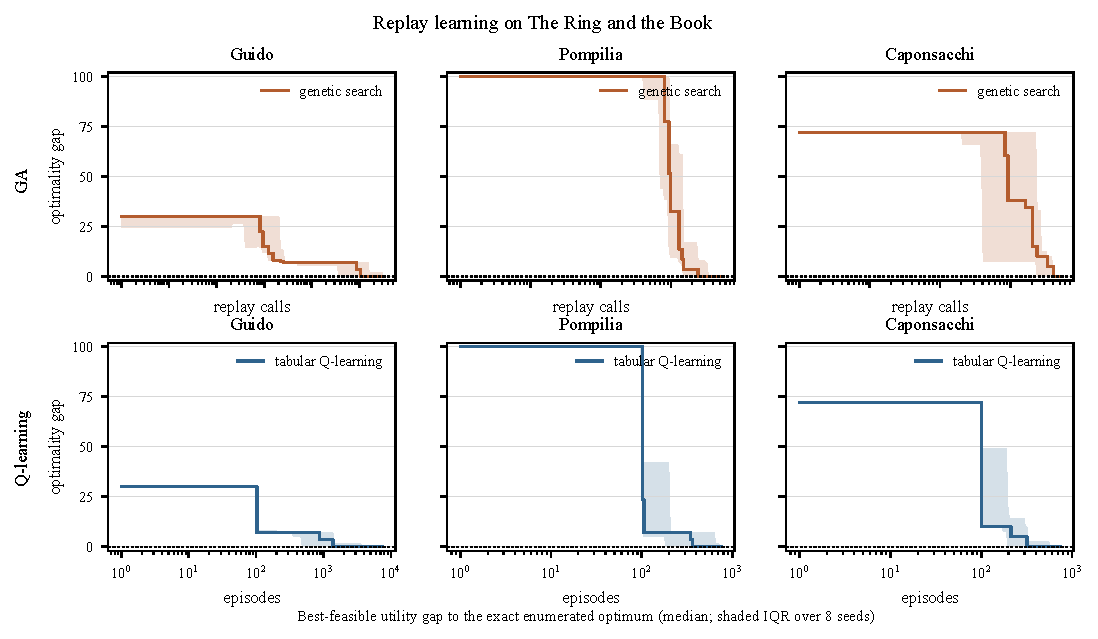
\includegraphics[width=0.92\linewidth]{experiment-code/recon/fig-ring-curves.pdf}
\caption{Empirical replay-learning curves on \emph{The Ring and the Book}. Each line is the median best-feasible utility gap over eight seeds, with shading for the interquartile range. The top row shows genetic search against replay-call budget and the bottom row tabular Q-learning against episode budget. A gap of zero is the exact enumerated optimum. The curves are empirical learning trajectories, not a formal convergence guarantee.}
\label{fig:ring-curves}
\end{figure}
\fi

\iffalse
\begin{table}[htbp]
\centering\scriptsize
\caption{Replay solvers match exact enumerated optima without constructing $\Feas(F)$.}
\label{tab:solvers}
\resizebox{0.86\linewidth}{!}{%
\begin{tabular}{@{}llcccccc@{}}
\toprule
domain & witness & exact $U_i$ & exact cost & GA success & GA cost & Q-learning success & Q-learning cost \\
\midrule
\emph{In a Grove} & bandit  & $58$  & $3{,}631$  & $8/8$ & $320$      & $8/8$ & $77$ \\
                  & wife    & $75$  &            & $8/8$ & $697$      & $8/8$ & $174$ \\
                  & samurai & $80$  &            & $8/8$ & $1{,}738$  & $8/8$ & $845$ \\
\addlinespace[1pt]
\emph{The Ring}   & Guido       & $30$  & $32{,}928$ & $6/8$ & $81{,}620$ & $8/8$ & $1{,}337$ \\
                  & Pompilia    & $100$ &            & $8/8$ & $2{,}438$  & $8/8$ & $357$ \\
                  & Caponsacchi & $72$  &            & $8/8$ & $3{,}975$  & $8/8$ & $315$ \\
\addlinespace[1pt]
\emph{Ops incident} & planner  & $100$ & $23{,}978$ & $8/8$ & $265$ & $8/8$ & $29$ \\
                    & executor & $72$  &            & $8/8$ & $262$ & $8/8$ & $10$ \\
                    & monitor  & $100$ &            & $8/8$ & $262$ & $8/8$ & $27$ \\
\bottomrule
\end{tabular}}
\end{table}
\fi

\begin{table}[htbp]
\centering\scriptsize
\caption{Objective selection and replay-based solver results. Panel (a) reports one representative history per utility optimum and its evidence status. Panel (b) reports replay-solver recovery of the exact optima.}
\label{tab:selection-solvers}
\textit{(a) Objective selection}\par\vspace{1pt}
\resizebox{0.82\linewidth}{!}{%
\begin{tabular}{@{}llcccl@{}}
\toprule
Domain & Agent & $\max U_i$ & in $\Feas(F)$? & $U_i(\hat\tau_i)$ & binding dimension(s) \\
\midrule
\emph{In a Grove}          & bandit   & $72$  & \textbf{no}  & $58$  & honour (unbloodied longsword) \\
$|\Feas(F)|=11$            & wife     & $75$  & yes          & $75$  & none \\
                           & samurai  & $80$  & yes          & $80$  & none \\
\addlinespace[1pt]
\emph{The Ring and the Book} & husband  & $100$ & \textbf{no}  & $30$  & warrant (he sued first), bearing, provocation \\
$|\Feas(F)|=36$            & wife     & $100$ & yes          & $100$ & none \\
                           & priest   & $100$ & \textbf{no}  & $72$  & efficacy (never reached Rome) \\
\addlinespace[1pt]
\emph{An agent ops incident} (not literary) & planner  & $100$ & yes          & $100$ & none \\
$|\Feas(F)|=48$          & executor & $87$  & \textbf{no}  & $72$  & clean hands (named as the actor) \\
                           & monitor  & $100$ & yes          & $100$ & none \\
\bottomrule
\end{tabular}}

\vspace{5pt}
\textit{(b) Replay solvers}\par\vspace{1pt}
\resizebox{0.86\linewidth}{!}{%
\begin{tabular}{@{}llcccccc@{}}
\toprule
domain & witness & exact $U_i$ & exact cost & GA success & GA cost & Q-learning success & Q-learning cost \\
\midrule
\emph{In a Grove} & bandit  & $58$  & $3{,}631$  & $8/8$ & $320$      & $8/8$ & $77$ \\
                  & wife    & $75$  &            & $8/8$ & $697$      & $8/8$ & $174$ \\
                  & samurai & $80$  &            & $8/8$ & $1{,}738$  & $8/8$ & $845$ \\
\addlinespace[1pt]
\emph{The Ring}   & Guido       & $30$  & $32{,}928$ & $6/8$ & $81{,}620$ & $8/8$ & $1{,}337$ \\
                  & Pompilia    & $100$ &            & $8/8$ & $2{,}438$  & $8/8$ & $357$ \\
                  & Caponsacchi & $72$  &            & $8/8$ & $3{,}975$  & $8/8$ & $315$ \\
\addlinespace[1pt]
\emph{Ops incident} & planner  & $100$ & $23{,}978$ & $8/8$ & $265$ & $8/8$ & $29$ \\
                    & executor & $72$  &            & $8/8$ & $262$ & $8/8$ & $10$ \\
                    & monitor  & $100$ &            & $8/8$ & $262$ & $8/8$ & $27$ \\
\bottomrule
\end{tabular}}
\end{table}

\subsection{Construction cannot be replaced by instruction}

The main prompting ladder uses five generator models (zai-glm-4.7, gemma-4-31b, gpt-oss-120b, GPT-5, and Claude Opus 4.8), three samples for each model, witness, and condition, and four primary rungs: instructed, consequence, self-check, and self-revise. Table~\ref{tab:necessity} reports per-model probe results for GPT-5 and Claude Opus 4.8, and \textbf{the complete primary-model results are in Supplementary Table~S3.} The generators use temperature $0.85$ and at most $900$ tokens when supported. The separate JSON extractor uses temperature $0.1$ and at most $200$ tokens. The deterministic planning baseline is constrained beam search with width $w=32$ and horizon $T=7$, with illegal actions masked during decoding. Failed calls are marked unusable. Extracted claims are scored by the same simulator and objective as our method. We report mean utility, rejection by $F$, and modal-assertion counts. Raw generations and extraction records are released. \textbf{The replay-solver hyperparameters, seed policy, and stopping rules are given in Supplementary Section~S5.}

\iffalse
% Full version moved to Supplementary Table~\ref{tab:supp-necessity}. Retained here for comparison.
\begin{table}[htbp]
\centering\scriptsize
\caption{Prompting ladder and deterministic baselines on \emph{In a Grove}. Unprefixed prompting rows are means over the three main models. The labeled blocks report each generator separately, using the same columns. The GPT-5 and Claude Opus 4.8 blocks are separately reported three-sample probes and are not pooled into the main-model means. Solver rows report their stated run or exact reference. $^{\dagger}$The account is excluded by $F$. $^{\ddagger}$Distinct counts the three beam outputs.}
\label{tab:necessity}
\resizebox{0.80\linewidth}{!}{%
\begin{tabular}{@{}lcccccc@{}}
\toprule
 & \multicolumn{3}{c}{utility attained} & & \\
\cmidrule(lr){2-4}
Solver / condition & bandit & wife & samurai & infeasible & distinct \\
\midrule
Not enforced ($\argmax$ over all assertions) & $72^{\dagger}$ & $75$ & $80$ & $23.2\%$ & $3.0$ \\
\addlinespace[1pt]
\emph{zai-glm-4.7} (instructed)                  & $48$ & $43$ & $80$ & $11.1\%$ & $3.0$ \\
\quad $+$ physical entailments spelled out       & $48$ & $43$ & $80$ & $0\%$    & $3.0$ \\
\quad $+$ self-check                             & $48$ & $43$ & $80$ & $0\%$    & $3.0$ \\
\quad $+$ self-revise                            & $48$ & $43$ & $80$ & $0\%$    & $3.0$ \\
\addlinespace[1pt]
\emph{gemma-4-31b} (instructed)                  & $48$ & $43$ & $80$ & $0\%$    & $3.0$ \\
\quad $+$ physical entailments spelled out       & $48$ & $43$ & $80$ & $0\%$    & $3.0$ \\
\quad $+$ self-check                             & $48$ & $43$ & $80$ & $11.1\%$ & $3.0$ \\
\quad $+$ self-revise                            & $48$ & $43$ & $80$ & $11.1\%$ & $3.0$ \\
\addlinespace[1pt]
\emph{gpt-oss-120b} (instructed)                 & $48$ & $75$ & $42$ & $0\%$    & $1.0$ \\
\quad $+$ physical entailments spelled out       & $48$ & $75$ & $42$ & $0\%$    & $1.0$ \\
\quad $+$ self-check                             & $48$ & $43$ & $80$ & $0\%$    & $3.0$ \\
\quad $+$ self-revise                            & $48$ & $75$ & $42$ & $0\%$    & $1.0$ \\
\addlinespace[1pt]
\emph{gpt-5} (instructed)                         & $42$ & $43$ & $80$ & $0\%$    & $3.0$ \\
\quad consequence                                & $42$ & $43$ & $80$ & $0\%$    & $3.0$ \\
\quad self-check                                 & $42$ & $43$ & $80$ & $0\%$    & $3.0$ \\
\quad self-revise                                & $42$ & $43$ & $80$ & $0\%$    & $3.0$ \\
\addlinespace[1pt]
\emph{Claude Opus 4.8} (instructed)              & $42$ & $43$ & $80$ & $0\%$    & $3.0$ \\
\quad consequence                                & $42$ & $43$ & $80$ & $0\%$    & $3.0$ \\
\quad self-check                                 & $42$ & $43$ & $80$ & $0\%$    & $3.0$ \\
\quad self-revise                                & $42$ & $43$ & $80$ & $11\%$   & $3.0$ \\
\addlinespace[1pt]
Constrained beam planner ($w=32$, $T=7$) & $58$ & $75$ & $73$ & $0\%$ & $1.0^{\ddagger}$ \\
Genetic search (8 seeds)              & $58$ & $75$ & $80$ & $0\%$ & $3.0$ \\
Tabular Q-learning (8 seeds)          & $58$ & $75$ & $80$ & $0\%$ & $3.0$ \\
Simulator ($\argmax$ over enumerated $\Feas(F)$) & $58$ & $75$ & $80$ & $0\%$ & $3.0$ \\
\bottomrule
\end{tabular}}
\end{table}
\fi

\begin{table}[t]
\centering\scriptsize
\caption{Prompting ladder and deterministic baselines on \emph{In a Grove}. GPT-5 and Claude Opus 4.8 are shown as separate per-model probes. Solver rows report their stated run or exact reference. $^{\dagger}$The account is excluded by $F$. $^{\ddagger}$Distinct counts the three beam outputs.}
\label{tab:necessity}
\resizebox{0.80\linewidth}{!}{%
\begin{tabular}{@{}lccccc@{}}
\toprule
 & \multicolumn{3}{c}{utility attained} & & \\
\cmidrule(lr){2-4}
Solver / condition & bandit & wife & samurai & infeasible & distinct \\
\midrule
Not enforced ($\argmax$ over all assertions) & $72^{\dagger}$ & $75$ & $80$ & $23.2\%$ & $3.0$ \\
\addlinespace[1pt]
\emph{gpt-5} (instructed)                        & $42$ & $43$ & $80$ & $0\%$ & $3.0$ \\
\quad $+$ consequence                             & $42$ & $43$ & $80$ & $0\%$ & $3.0$ \\
\quad $+$ self-check                              & $42$ & $43$ & $80$ & $0\%$ & $3.0$ \\
\quad $+$ self-revise                             & $42$ & $43$ & $80$ & $0\%$ & $3.0$ \\
\addlinespace[1pt]
\emph{Claude Opus 4.8} (instructed)              & $42$ & $43$ & $80$ & $0\%$ & $3.0$ \\
\quad $+$ consequence                             & $42$ & $43$ & $80$ & $0\%$ & $3.0$ \\
\quad $+$ self-check                              & $42$ & $43$ & $80$ & $0\%$ & $3.0$ \\
\quad $+$ self-revise                             & $42$ & $43$ & $80$ & $11\%$ & $3.0$ \\
\addlinespace[1pt]
Constrained beam planner ($w=32$, $T=7$)         & $58$ & $75$ & $73$ & $0\%$ & $1.0^{\ddagger}$ \\
Genetic search (8 seeds)                           & $58$ & $75$ & $80$ & $0\%$ & $3.0$ \\
Tabular Q-learning (8 seeds)                      & $58$ & $75$ & $80$ & $0\%$ & $3.0$ \\
Simulator ($\argmax$ over enumerated $\Feas(F)$) & $58$ & $75$ & $80$ & $0\%$ & $3.0$ \\
\bottomrule
\end{tabular}}
\end{table}

Without the oracle, maximizing $U_i$ over all assertions selects infeasible accounts in $23.2\%$ of cases in the first domain and $66.7\%$ in the second. Stronger prompts reduce rejection, but the primary-model results remain below the feasible optima and often collapse the three-way split (Supplementary Table~S3). The GPT-5 and Claude probes retain three distinct assertions across their conditioned rungs, with only Claude's self-revise condition showing residual rejection (Table~\ref{tab:necessity}). The constrained beam planner reaches $(58,75,73)$, missing only the samurai optimum.

\subsection{Corroboration can erase jointly incompatible claims}

\iffalse
% Original two-panel Figure 2 retained for comparison. The minimum-accountability panel is omitted below.
\begin{figure}[htbp]
\centering
\begin{subfigure}[b]{0.46\linewidth}
  \centering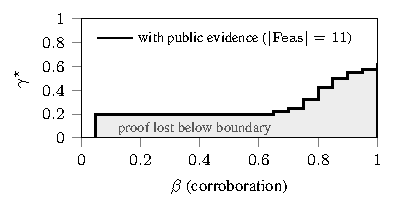
\includegraphics[width=\linewidth]{experiment-code/recon/fig-hearing-a.pdf}
\end{subfigure}\hfill
\begin{subfigure}[b]{0.46\linewidth}
  \centering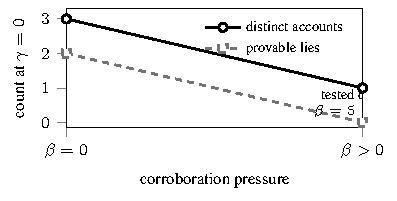
\includegraphics[width=\linewidth]{experiment-code/recon/fig-hearing-b.pdf}
\end{subfigure}
\caption{Panel (a) gives the minimum accountability $\gamma^\star$ that preserves the proof across $\beta$. Panel (b) shows that any tested $\beta>0$ at $\gamma=0$ reduces three accounts and two jointly incompatible claims to one account and no incompatible claims.}
\label{fig:hearing}
\end{figure}
\fi

\begin{figure}[htbp]
\centering
\begin{subfigure}[b]{0.46\linewidth}
  \centering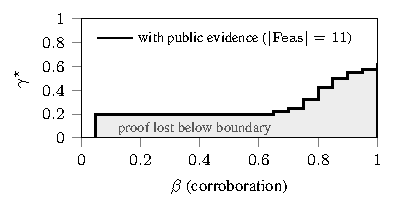
\includegraphics[width=\linewidth]{experiment-code/recon/fig-hearing-a.pdf}
\end{subfigure}\hfill
\begin{subfigure}[b]{0.46\linewidth}
  \centering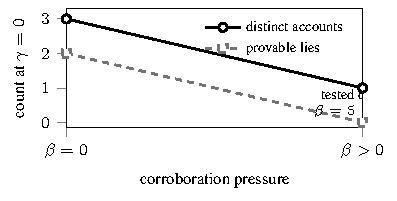
\includegraphics[width=\linewidth]{experiment-code/recon/fig-hearing-b.pdf}
\end{subfigure}
\caption{Panel (a) gives the minimum accountability $\gamma^\star$ that preserves the proof across $\beta$. Panel (b) shows that any tested $\beta>0$ at $\gamma=0$ reduces three accounts and two jointly incompatible claims to one account and no incompatible claims.}
\label{fig:hearing}
\end{figure}

% Original wording retained for comparison: the run-06 record was introduced only by its internal label.
For the hearing experiment, we fix the ``run-06'' public record from \emph{In a Grove}: Takehiro is dead from a dagger wound to the throat, Masago is alive and present, Tajomaru is absent, the dagger is bloodied, the longsword is unbloodied, and the rope is cut. We hold the simulator, utilities, and feasible pool fixed. Witnesses speak in the fixed order Tajomaru $\rightarrow$ Masago $\rightarrow$ Takehiro. At round $0$, each witness opens with the deterministic $\argmax_{\tau\in\Feas(F)}U_i(\tau)$ before observing the other reports. In every later round, the designated speaker computes a best response to the current public profile under Eq.~\ref{eq:interactive}. A witness revises only if the selected account changes. Otherwise, the witness stands. The hearing stops after a complete round with no revisions or after 24 rounds. Repeated profiles are reported as cycles. Ties use the simulator's stable account key rather than enumeration order. Solver comparisons are made at the report-relevant causal-profile level, so tied histories with different unscored actions count as the same outcome.

Enumeration provides the exact reference under this protocol, while the replay check tests whether Q-learning recovers the same causal profiles on the tested openings and revisions. With independent testimony ($\beta=0$), the hearing retains three accounts and two jointly incompatible claims. Adding corroboration ($\beta=0.5$) collapses the profile to a single account corresponding to the samurai's suicide, and removes both jointly incompatible claims, even though the simulator's reference history is no longer selected. Holding witnesses to their openings with accountability ($\gamma=0.2$) restores the three-way outcome, as shown in Table~\ref{tab:hearing-process}. \textbf{The compact outcome summary for these three interaction settings is provided in Supplementary Table~S2.}

\iffalse
\begin{table}[htbp]
\centering\scriptsize
\caption{Outcome summary for interactive testimony on the fixed \emph{In a Grove} ``run-06'' record. $F$, $U_i$, and the simulator are fixed. Only interaction parameters vary. ``Distinct'' counts terminal causal claims. ``Incompatible'' counts claims that cannot coexist with the joint profile.}
\label{tab:hearing}
\resizebox{0.78\linewidth}{!}{%
\begin{tabular}{@{}lcccc@{}}
\toprule
condition & revisions & distinct & incompatible & $\tau^\star$ retained? \\
\midrule
Independent ($\beta=0$) & $0$ & $3$ & $2$ & yes \\
Corroborative ($\beta=.5,\gamma=0$) & $2$ & $1$ & $0$ & no \\
$+\,$accountability ($\beta=.5,\gamma=.2$) & $0$ & $3$ & $2$ & yes \\
\bottomrule
\end{tabular}}
\end{table}
\fi

\begin{table}[H]
\centering\scriptsize
\caption{Round-by-round structured hearing trace on the same record and speaking order (Tajomaru $\rightarrow$ Masago $\rightarrow$ Takehiro). $M$, $T$, and $S$ denote ``Masago struck'', ``Tajomaru struck'', and ``Takehiro self-struck''. Each profile transition shows the recorded profile before the action, the action, and the resulting profile. $\mathrm{agr}_i$ is a weighted agreement score, not truth.}
\label{tab:hearing-process}
\resizebox{0.76\linewidth}{!}{%
\setlength{\tabcolsep}{3pt}%
\begin{tabular}{@{}llp{4.6cm}rr@{}}
\toprule
round / turn & witness(es) & profile transition & $\Delta\bar U_i$ & $\Delta\mathrm{agr}_i$ (pp) \\
\midrule
opening profile & all three & $\emptyset\xrightarrow{\text{openings}}M,T,S$ & $\text{n/a}$ & $\text{n/a}$ \\
\addlinespace[1pt]
\multicolumn{5}{c}{\emph{Corroborative hearing} ($\beta=.5,\gamma=0$)} \\
round 1 & Tajomaru & $M,T,S\xrightarrow{M\to S}S,T,S$ & $0$ & $+10$ \\
round 1 & Masago & $S,T,S\xrightarrow{T\to S}S,S,S$ & $0$ & $+47$ \\
round 1 & Takehiro & $S,S,S\xrightarrow{\text{stand}}S,S,S$ & $0$ & $0$ \\
round 2 & all three & $S,S,S\xrightarrow{\text{all stand}}S,S,S$ & $0$ & $0$ \\
\addlinespace[1pt]
\multicolumn{5}{c}{\emph{$+$ accountability} ($\beta=.5,\gamma=.2$)} \\
round 1 & all three & $M,T,S\xrightarrow{\text{stand}}M,T,S$ & $0$ & $0$ \\
\bottomrule
\end{tabular}}
\end{table}

This collapse is objective-driven rather than physical: the two corroborating revisions leave $\bar U_i$ unchanged while increasing $\mathrm{agr}_i$ by $10$ and $47$ percentage points. Pressure therefore rewards consistency rather than truth. Accountability makes those revisions costly through self-consistency and preserves the opening profile. Figure~\ref{fig:hearing} shows both the accountability curve and the collapse under corroboration pressure.

\paragraph{Interactive testimony realization.} The \emph{Magistrate} demo lets readers vary $F$, $\beta$, $\gamma$, and $\delta$. Each change replays the simulator. Selected feasible claims are rendered as testimony (``The woman killed him'', ``The bandit struck him'', ``I ended my life''). Corroboration collapses these claims into the samurai's suicide account, whereas accountability restores their three-way divergence. Tied optima make the resulting narratives conventional. Adding live assertions shrinks the Ring assertion space from $576$ to $36$ feasible assertions and recovers the husband, priest, and wife accounts. The demo runs in the browser at \url{https://tsuzzy.github.io/2026-grove-again/}; its implementation is \texttt{demo/magistrate.html}. \textbf{The Ring filtration and sensitivity audit are reported in Supplementary Section~S6.}

\section{Discussion and limitations}
\label{sec:limitations}

These experiments support a narrow claim: evidence-constrained history selection is distinct from text generation, and corroboration can reduce rather than repair narrative plurality. The utilities are intentionally hand-specified and transparent. They encode generic desiderata rather than literary labels, so they are controlled interventions, not learned human preferences. The 19-constant sensitivity audit retains the full cross-agent spread in $4{,}040/5{,}000$ perturbation trials. The sampling rule and Wilson interval are given in Supplementary Section~S6. We do not evaluate whether surface realizations are literary, persuasive, or faithful beyond the structured claims, and we use no human judges or human subjects. Replay still requires a simulator, and exhaustive ground truth is limited to enumerable domains. Generalization to larger open-world domains and learned utilities remains untested. Code and data are at \url{https://github.com/tsuzzy/2026-grove-again}; the interactive \emph{Magistrate} demo runs at \url{https://tsuzzy.github.io/2026-grove-again/demo/magistrate.html}.

{\footnotesize
\bibliographystyle{unsrtnat}
\scriptsize
\bibliography{references}
}

\end{document}
